\documentclass{beamer}
%\documentclass[handout,t]{beamer}

\batchmode
% \usepackage{pgfpages}
% \pgfpagesuselayout{4 on 1}[letterpaper,landscape,border shrink=5mm]

\usepackage{amsmath,amssymb,color}

\usetheme{Berlin}
\usecolortheme{bear}

\title{Implementation of elliptic curve cryptography in constrained environments}
\author[Anthony Van Herrewege]{Anthony Van Herrewege\\Prof. Dr. Ir. I. 	Verbauwhede \& Prof. Dr. Ir. B. Preneel}
\date{18 Februari 2009}
%\pgfdeclareimage[height=1cm]{brown-logo}{brown-logo.pdf}
%\logo{\pgfuseimage{brown-logo}\hspace*{0.3cm}}

\AtBeginSection[]
{
  \begin{frame}<beamer>
    \frametitle{Outline}
    \tableofcontents[currentsection]
  \end{frame}
}
\beamerdefaultoverlayspecification{<+->}

\begin{document}

\frame{\titlepage}

\section[Outline]{}
\begin{frame}{Outline}
  \tableofcontents
\end{frame}

\section{Introduction}
\subsection*{Introduction}
\begin{frame}
	\begin{center}
		Implement a \alert{compact} \alert{hardware} implementation of \alert{elliptic curve pairings}.
		
		\begin{itemize}
			\item<2-> Program in GEZEL
			\item<2-> Optimize in VHDL
			\item<2-> Synthetize to FPGA/ASIC
		\end{itemize}
	\end{center}
\end{frame}

\section{Elliptic Curve Pairings}
\subsection*{Elliptic Curve Pairings}
\begin{frame}{Overview}
	\begin{enumerate}
		\item<1-> What?
		\item<1-> Why?
		\item<1-> How?
	\end{enumerate}
\end{frame}

\begin{frame}{What?}
  \begin{itemize}
    \item<1-> Public key cryptography
    \item<2-> \alert{Identity}-based cryptography
    \item<3-> Calculations over elliptic curves
  \end{itemize}
\end{frame}

\begin{frame}{Why?}
	\begin{itemize}
  		\item<1-> Identity-based cryptography\\
  			\begin{itemize}
				\item<1-> No public key lookup required:\\
					$\quad$eg. $P$ = National identification number
				\item<2-> Date-stamped encryption possible:\\
					$\quad$eg. $P$ = Nin + "20091223"
				\item<3-> Other positive aspects:\\
					$\quad$Non-interactive key establishment\\
					$\quad$Single round tripartite key establishment\\
					$\quad$Ideal for eg. sensor networks
				\item<4-> Drawbacks as well:\\
					$\quad$no key revocation, still a central authority, $\ldots$
			\end{itemize}
		\item<5-> Key strength comparison [bits]:\\
			\begin{tabular}{ll}
				RSA			&	3072\\
				\alert{ECC}	&	\alert{256}\\
			\end{tabular}
	\end{itemize}
\end{frame}

%\begin{frame}{How? - Underlying mathematics}
%	\begin{itemize}
%		\item<1-> Discrete logarithm (DL) problem [hard]:\\
%				\[\text{Given: } g, h \in G \colon h \overset{?}{=} g^a \pmod n\]
%		\item<2-> Computational DL problem [hard]:\\
%				\[\text{Given: } g, g^a, g^b, \in G \colon h \overset{?}{=} g^{ab} \pmod n\]
%		\item<3-> Decision DL problem [easy]:\\
%				\[\text{Given: } g, g^a, g^b, g^c \in G \colon g^c \overset{?}{=} g^{ab} \pmod n \]
%	\end{itemize}
%\end{frame}

\begin{frame}{How?}
	Elliptic curve pairing $e$:
	
	\[ e : G_1 \times G_1 \rightarrow G_2 \]
	
	Mapping needs to be:
	
	\begin{itemize}
		\item<1-> Bilinear: $e(P_1 + P_2, P_3) = e(P_1, P_3) \cdot e(P_2, P_3)$
		\item<1-> Non-degenerate: $e(P, P) \neq 1$
		\item<1-> Efficiently computable
	\end{itemize}
	
	Several available pairings:\\
	
	\begin{center}Weil, \alert{Tate}, ate, eta, $\ldots$\end{center}
\end{frame}

\section{Implementation}
\subsection*{Implementation}
\begin{frame}{MALU}
	Modulo Arithmetic Logical Unit [general]:\\[8mm]
	\begin{center}
		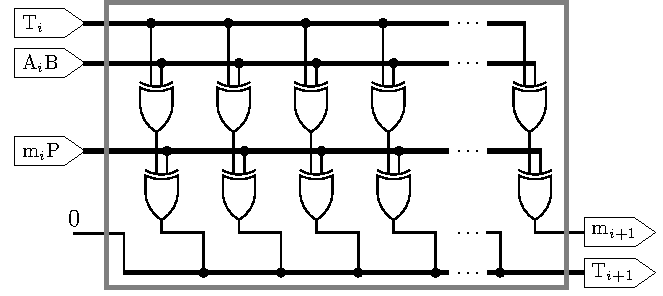
\includegraphics[height=0.5\paperheight]{images/malu-core-basic}
	\end{center}
\end{frame}

\begin{frame}{MALU}
	Modulo Arithmetic Logical Unit [optimized]:\\[3mm]
	\begin{center}
		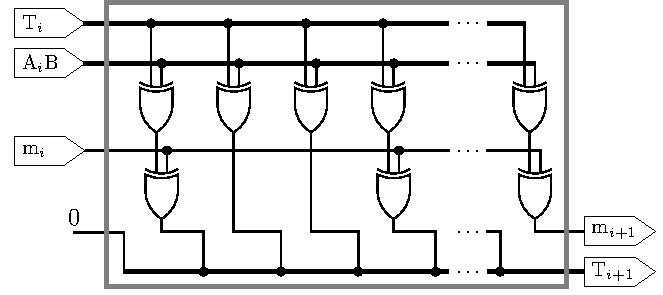
\includegraphics[height=0.5\paperheight]{images/malu-core-optimized}
	\end{center}
\end{frame}

\begin{frame}{MALU}
	Modulo Arithmetic Logical Unit [optimized; d-bits wide]:\\
	\begin{center}
		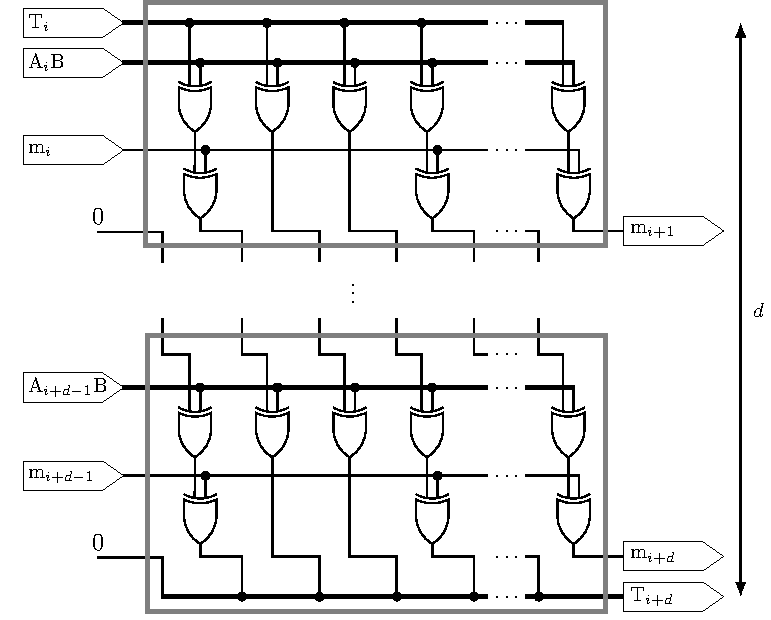
\includegraphics[height=0.55\paperheight]{images/malu-core-optimized-d}
	\end{center}
\end{frame}

\begin{frame}{Wrappers - $GF_{2^m}$}
	$GF_{2^m}$ Multiplication/Addition:\\
	\begin{center}
		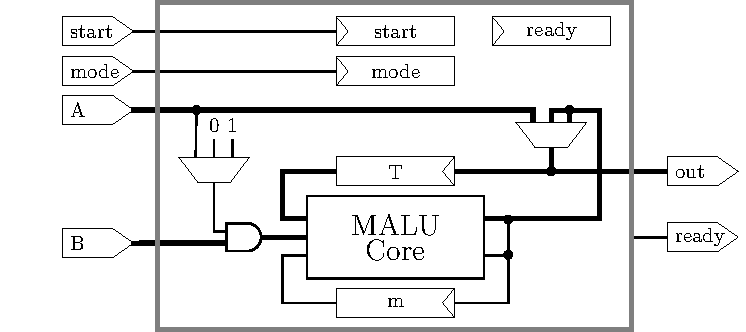
\includegraphics[height=0.55\paperheight]{images/malu-wrapper-gf2m}
	\end{center}
\end{frame}

\begin{frame}{Wrappers - ECC}
	ECC Point Addition/Doubling:\\
	\begin{center}
		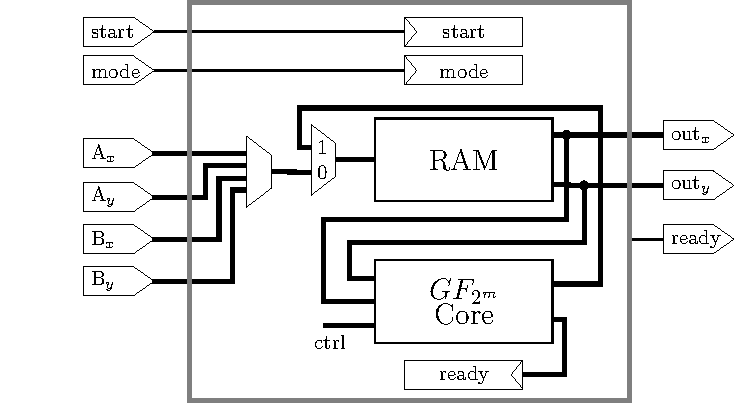
\includegraphics[height=0.55\paperheight]{images/malu-wrapper-ecc}
	\end{center}
\end{frame}

\begin{frame}{State of the art}
	Some currently available implementations:\\
	
	\begin{center}
	\begin{tabular}{llll}
		Name		&	Platform	&	Field	&	Speed\\
		\hline
		TinyTate		&	ATMega128L [7.4Mhz]	& $\mathbb{F}_{2^{256}}$	& 30.2s\\
		TinyPBC		&	ATMega128L [7.4Mhz]	& $\mathbb{F}_{2^{256}}$	& 5.45s\\
		Hankerson	&	P4 [2.8Ghz]				& $\mathbb{F}_{2^{1223}}$	& 0.07s\\
		Hankerson	&	P4 [2.8Ghz]	(SSE) 	& $\mathbb{F}_{2^{1223}}$	& 0.03s\\
		\end{tabluar}
	\end{center}
\end{frame}

\section{Conclussion}
\subsection*{Conclussion}
\begin{frame}{Progress so far}
	\begin{itemize}
		\item<1-> MALU
		\item<1->	$GF_{2^m}$ functions
		\item<1-> ECC functions
		\item<1-> Pairing functions (partial)
	\end{itemize}
\end{frame}

\begin{frame}{To do}
	\begin{itemize}
		\item<1-> Complete pairing functions
		\item<1-> Bugfixing
		\item<1-> Optimization (VHDL)
		\item<1-> Write thesis text
	\end{itemize}
\end{frame}

\begin{frame}{The end}
	\begin{center}\LARGE Questions?\end{center}
\end{frame}

\end{document}
